\documentclass[final, dvipdfmx]{beamer}
\usepackage[
	orientation=portrait,
	size=a0paper,
	scale=1.4,
	debug
	]{beamerposter}
\mode<presentation>{
	\usetheme{singapore}
	\useoutertheme{infolines}
	\usecolortheme{rose} % いじらない
	\usefonttheme{professionalfonts}
	\useinnertheme{rectangles}
	\useoutertheme{tree}
}
% 日本語(非英語)に対応
\usepackage[japanese]{babel}
% ポスターで不要な要素の非表示
\setbeamertemplate{navigation symbols}{}
\setbeamertemplate{headline}{}
\setbeamertemplate{footline}{}
% 日本語をゴシック体
\renewcommand{\kanjifamilydefault}{\gtdefault}
% blockの色の設定
%\setbeamercolor{block body}{bg=white, fg=black} % tcbsetforeverylayer とかでやったほうがいいかも
% フォントの大きさの設定
%\setbeamerfont{caption}{size=\normalsize}
\setbeamerfont{block title}{size=\LARGE}
\setbeamerfont*{itemize/enumerate body}{size=\normalsize}
\setbeamerfont*{itemize/enumerate subbody}{parent=itemize/enumerate body, size=\normalsize}
\setbeamerfont*{itemize/enumerate subsubbody}{parent=itemize/enumerate subbody, size=\normalsize}
% 箇条書きのアイコンを変更
\setbeamertemplate{itemize item}[circle]
\setbeamertemplate{enumerate items}[default]
\setbeamertemplate{itemize subitem}[triangle]
%\setbeamercolor{enumerate item}{fg=black}
% 参考文献のアイコンを標準のに
\setbeamertemplate{bibliography item}[text]
% 参考文献の文字色を変更
\setbeamercolor*{bibliography item}{fg=black}
\setbeamercolor*{bibliography entry author}{fg=black}
\setbeamercolor*{bibliography entry title}{fg=black}
\setbeamercolor*{bibliography entry location}{fg=black}
% Beamer-blockの実装をtcolorboxで行う、TeX Live 2024が必要
\useinnertheme[rounded]{tcolorbox}
\tcbsetforeverylayer{
  frame style={draw=block title.bg, line width=4mm}
}

% 数式
\usepackage{amsmath}
\usepackage{amssymb}
\usepackage{physics}
\usepackage{mathtools}
% 行列の表現を拡張する、まだよくわかっていない
\usepackage{nicematrix}
% 画像・表
\usepackage{graphicx}
\usepackage{color}
\usepackage{here}
% 図表のcaptionを設定
\usepackage{caption}
\usepackage[subrefformat=parens]{subcaption}
\captionsetup[figure]{name=図}
\captionsetup[table]{name=表}
\setbeamertemplate{caption}[numbered]
% 画像フォルダへのパスを追加
\graphicspath{ {fig/} }
% 行間
%\usepackage{setspace} % algorithmのキャプションが崩れる
% 疑似コード
\usepackage{algorithm}
\usepackage{algorithmicx}
\usepackage{algpseudocode}
\algnewcommand{\IIf}[1]{\State\algorithmicif\ #1\ \algorithmicthen}
\algnewcommand{\EndIIf}{\unskip\ \algorithmicend\ \algorithmicif}
% タイトルの背景に色を付けるために使用
\usepackage{tcolorbox}
% コメントアウト
\usepackage{comment}
% ダミーテキスト
\usepackage{lipsum}
% PDFのメタ情報・URL
\usepackage{hyperref}
\usepackage{pxjahyper}
\hypersetup{
	setpagesize=false,
	bookmarks=true,
	bookmarksdepth=tocdepth,
	bookmarksnumbered=true,
	hidelinks,
	hyperfootnotes=false,
	pdftitle={シフト線形方程式に対するMINRES法の適用と性能評価},
	pdfsubject={電気通信大学大学院修士課程中間発表},
	pdfauthor={日高 俊太郎},
	pdfkeywords={シフト線形方程式, Krylov部分空間法, MINRES法, 並列化, 高性能計算}
}

% コマンドの設定
\newcommand{\equref}[1]{(\ref{#1})}					% 括弧で囲まれた参照
\newcommand{\Equref}[1]{式(\ref{#1})}				% 数式の参照
\newcommand{\Tabref}[1]{表\ref{#1}}					% 表の参照
\newcommand{\Figref}[1]{図\ref{#1}}					% 図の参照
\renewcommand{\top}[0]{\mathrm{T}}					% 転置
\newcommand{\htop}[0]{\mathrm{H}}					% Hermite転置
\renewcommand{\i}[0]{\mathrm{i}}					% 虚数単位
\newcommand{\KS}[3]{\mathcal{K}_{#1}({#2}, {#3})}			% Krylov Subspace
\newcommand{\inpro}[2]{\langle #1, #2 \rangle}			% 内積
\newcommand{\conj}[1]{\overline{#1}}					% 複素共役
% itemizeのシンボルをitemize外で使えるようにする
% https://tex.stackexchange.com/questions/519279/beamer-bullets-without-itemize/519318#519318
%\newcommand{\myitem}{\par\leavevmode\hskip\leftmarginii \hbox to\labelwidth{\hss\usebeamercolor[fg]{itemize subitem}\usebeamertemplate{itemize subitem}}\hspace{\labelsep}}
\newcommand{\myitem}{
	\leavevmode\hskip\leftmarginii \hbox to
	\labelwidth{\hss\usebeamercolor[fg]{itemize subitem}\usebeamertemplate{itemize subitem}}
}

% 行間の設定
\renewcommand{\baselinestretch}{1.2}
% 数式の上下のスペースの変更
\AtBeginDocument{
  \abovedisplayskip     = 0.6\abovedisplayskip
  \abovedisplayshortskip= 0.6\abovedisplayshortskip
  \belowdisplayskip     = 0.6\belowdisplayskip
  \belowdisplayshortskip= 0.6\belowdisplayshortskip
}


\begin{document}

\begin{frame}[t]{}
	
% 色の設定は Beamer theme rose から取ってきた
% c:/texlive/2020/texmf-dist/tex/latex/beamer/beamercolorthemerose.sty

%\vspace{-0.76\baselineskip}
\vspace{-0.6\baselineskip}
\begin{tcolorbox}[
		colback=structure.fg,
		colframe=white,
		top=0mm,
		bottom=0mm,
		left=0mm,
		right=0mm
	]
\color{white}{
	\vspace{0.6\baselineskip}
	\begin{center}
		{\Huge シフト線型方程式に対するMINRES法の適用と性能評価}
	\end{center}
	\vspace{0.5\baselineskip}
	\begin{minipage}[]{0.8\columnwidth}
		\hspace{39cm} {\Large 日高 俊太郎$^*$}
		\vspace{0.2\baselineskip}\\
		\hspace{25.5cm} {\small $^*$ 電気通信大学 情報理工学研究科 情報・ネットワーク工学専攻 山本有作研究室}
	\end{minipage}
	\begin{minipage}[]{0.19\columnwidth}
		\begin{figure}\centering
			
\includegraphics[width=\columnwidth]{uec.png}
		\end{figure}
	\end{minipage}
}
\end{tcolorbox}



	\vspace{-\baselineskip}
	\begin{columns}[T]
	\begin{column}{.49\linewidth}
		\begin{block}{研究目的}
			\vspace{0.2\baselineskip}
			

本研究では,標準シフト線型方程式
\begin{align}
	(A + \sigma^{(k)}I)\vb{x}^{(k)} = \vb{b}, \qquad (k=1,\dots,M).
	\label{eq-std-sls}
\end{align}
に対する解法である shifted MINRES法\cite{ref-S-HIDAKA-2025}の効率的な計算モデルの検討を行う.\\
行列 $A$ は\textcolor{red}{実対称}・\textcolor{red}{エルミート}行列で $\sigma_{k}$ は\textcolor{red}{複素数},$I$ は\textcolor{red}{単位行列}であるとする.

		\end{block}
		\begin{block}{研究背景}
			\vspace{0.2\baselineskip}
			
標準シフト線型方程式 \eqref{eq-std-sls} は,量子力学や電子構造計算などに現れる.  
特に近年では,行列関数の計算における部分問題としても重要性が増している.

こうした問題では,\textcolor{red}{$10^7$~$10^8$次元を超える超大規模行列}が登場することもあり,従来の逐次的な解法では対応が困難である.

このような制約下では,次のような特性を持つアルゴリズムが求められる:
\begin{itemize}\setlength{\itemsep}{0pt}
  \item Matrix--free(行列全体を保持しない)
  \item 複数シフトに対する同時解法
  \item 並列計算への適用可能性
\end{itemize}
このような要請に応える手法として,Krylov部分空間法が注目されている.

		\end{block}
		\begin{block}{shifted MINRES法}
			\vspace{0.2\baselineskip}
			
MINRES法は,実対称またはエルミートな係数行列に対して有効な Krylov 部分空間法であり,
\textcolor{red}{Lanczos過程}に基づいて最小残差解を反復的に求める.

これをシフト線形方程式に拡張したのが shifted MINRES 法である.

アルゴリズムの概要: 
\vspace{-8pt}
\begin{enumerate}
	\item $A$に対して Lanczos過程を実行し,正規直交基底を構成
		\begin{align}
			\hspace{-2cm}
			AV_{n} = V_{n+1}\widehat{T}_{n},\ V_{n}=[\vb{v}_1 \ \cdots \ \vb{v}_n],\ T_{n} =
			{\small
			\begin{bNiceMatrix}[nullify-dots, columns-width=1.5em, cell-space-top-limit=5pt, cell-space-bottom-limit=5pt]
				\alpha_{1}	& \beta_{1}	&		&			\\
				\beta_{1}	& \Ddots	& \Ddots	& 			\\
    						& \Ddots	&		& \beta_{n-1}	\\
    						&		& \beta_{n-1}& \alpha_{n}		\\
			\end{bNiceMatrix}
			}
			,\ \widehat{T}_{n} = 
			{\small
			\mqty[T_{n} \\ \beta_{n}\vb{e}_{n}^{\top}]
			}
		\end{align}
	\item $k=1, 2, \dots, M$
	\begin{enumerate}
		\item $\widehat{T}_{n}^{(k)} = \widehat{T}_{n} + \sigma^{(k)} {\small \mqty[I \\ \vb{0}^\top]}$とおく($(A+\sigma^{(k)}I)V_{n}=V_{n+1}\widehat{T}_{n}^{(k)}$が成り立つ)
		\item $\widehat{T}_{n}^{(k)}$のQR分解を計算する($T_{n}^{(k)} = Q_n R_n$)
		\item $\vb{y}_{n}^{(k)} = \norm{\vb{b}} R_{n}^{-1} Q_{n}^{\htop} \vb{e}_{1}$を求める
			\begin{align}
				\| \vb{r}_n^{(k)} \|
				= \| \vb{b} - (A+\sigma_{k}I)\vb{x}_{n} \|
				&= \Bigl\| V_{n+1} \left( \|\vb{b}\| \vb{e}_1 - \widehat{T}_{n}^{(k)} \vb{y}_{n}^{(k)} \right) \Bigr\| \notag\\
				&= \Bigl\| \|\vb{b}\| \vb{e}_1 - \widehat{T}_{n}^{(k)} \vb{y}_{n}^{(k)} \Bigr\|
				\label{03-siki}
			\end{align}
		\item 最小残差解 $\vb{x}_{n}^{(k)} = V_{n} \vb{y}_{n}^{(k)}$を求める
	\end{enumerate}
\end{enumerate}
特徴:
\begin{itemize}
	\item \textcolor{red}{$1$回}のLanczos過程で\textcolor{red}{$M$個}の方程式に必要な基底が得られる
	\item \textcolor{red}{残差のノルムの単調減少性}と\textcolor{red}{無破綻性}を持つ
	\item シフトごとに\textcolor{red}{独立に}最小残差解を求められる
\end{itemize}

\vspace{0.5em}
\begin{figure}[H]
	\centering
	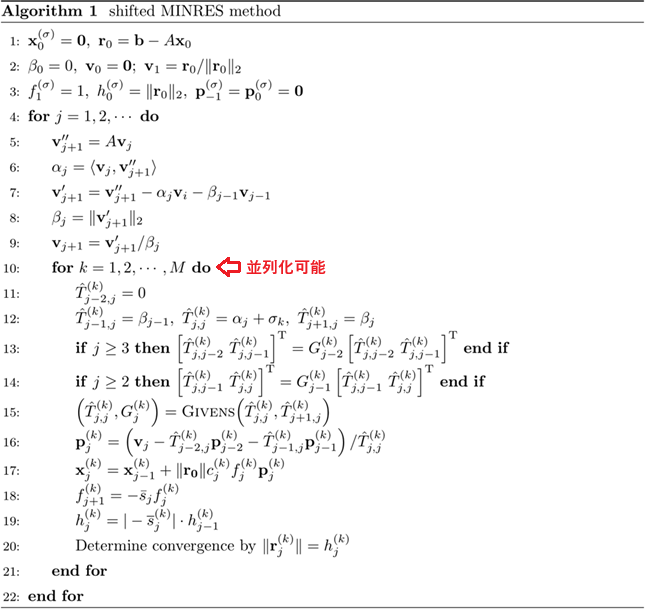
\includegraphics[scale=2.2]{./fig/algorithm-sminres.png}
\end{figure}



\begin{comment}
\begin{algorithm}[H]
	\caption{Multiply shifted MINRES algorithm}\label{Algorithm2}
	\begin{algorithmic}[1]
		\State ${\bf r}_0={\bf b}$, \, ${\bf q}_1 = {\bf r}_0/\|{\bf r}_0\|$, \, ${\bf p}_{-1}^{(m)}={\bf p}_0^{(m)}={\bf 0}$ \; ($m=1,\ldots,M$)
		\State $\beta_0=0$, \, $f_1^{(0,m)}=1$, \, $h_1^{(0,m)} = \|{\bf r}_0\|$ \; ($m=1,\ldots,M$)
		\For{$j=1, 2, \ldots,$}
			\State ${\bf q}_{j+1}^{\prime\prime} = A{\bf q}_j - \beta_{j-1}{\bf q}_{j-1}$
			\State $\alpha_j=\langle{\bf q}_{j+1}^{\prime\prime},{\bf q}_j\rangle$
			\State ${\bf q}_{j+1}^{\prime}={\bf q}_{j+1}^{\prime\prime}-\alpha_j{\bf q}_j$
			\State $\beta_j=\|{\bf q}_{j+1}^{\prime}\|$
			\For{$m=1,\ldots,M$}
				\State $r_{j-2,j}^{(m)}=0, \, r_{j-1,j}^{(m)}=\beta_{j-1}, \, r_{jj}^{(m)}=\alpha_j+\sigma^{(m)}$
				\State {\bf If} $j\ge 3$, update $r_{j-2,j}^{(m)}$ and $r_{j-1,j}^{(m)}$ by \eqref{eq:rkm2k}
				\State {\bf if} $j\ge 2$, update $r_{j-1,j}^{(m)}$ and $r_{jj}^{(m)}$ by \eqref{eq:rkm1k}
				\State compute $G_j^{(m)}$ and update $r_{jj}^{(m)}$ by \eqref{eq:rkk}
				\State ${\bf p}_j^{(m)}=({\bf q}_j-r_{j-2,j}^{(m)}{\bf p}_{j-2}^{(m)}-r_{j-1,j}^{(m)}{\bf p}_{j-1}^{(m)})/r_{jj}^{(m)}$
				\State ${\bf x}_j^{(m)}={\bf x}_{j-1}^{(m)} + \|{\bf r}_0\|c_j^{(m)} f_j^{(j-1,m)}{\bf p}_j^{(m)}$
				\State $f_{j+1}^{(j,m)}= -\bar{s}_j^{(m)} f_j^{(j-1,m)}$
				\State $h_{j+1}^{(j,m)}=|-\bar{s}_j^{(m)}| h_j^{(j-1,m)}$
			\EndFor
			\State ${\bf q}_{j+1}={\bf q}_{j+1}^{\prime}/\beta_j$
		\EndFor
	\end{algorithmic}
\end{algorithm}
\end{comment}
		\end{block}
	\end{column}
	\hspace{0.0\columnwidth}
	\begin{column}{.49\linewidth}
		\begin{block}{shifted MINRES法の並列化モデル}
			\vspace{0.2\baselineskip}
			


\begin{figure}[H]
	\begin{center}
		\begin{minipage}[]{0.49\columnwidth}
			\centering
			\colorbox{white}{ 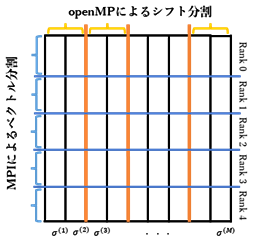
\includegraphics[scale=1.8]{./fig/parallel-model1.png} }
			\caption{並列化モデル1}
			\label{fig-parallel-model1}
		\end{minipage}
		\begin{minipage}[]{0.49\columnwidth}
			\centering
			\colorbox{white}{ 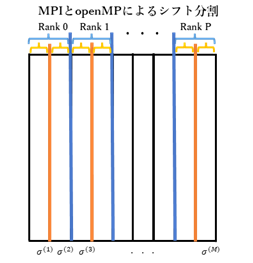
\includegraphics[scale=1.8]{./fig/parallel-model2.png} }
			\caption{並列化モデル2}
			\label{fig-parallel-model2}
		\end{minipage}
	\end{center}
\end{figure}

		\end{block}
		\begin{block}{数値実験}
			\vspace{0.2\baselineskip}
			

実行時間の比較

逐次 : モデル1 : モデル2
		\end{block}
		\begin{block}{まとめと今後の展望}
			\vspace{0.2\baselineskip}
			

\begin{itemize}
	\item shifted MINRES法に対する2種類の並列化モデルの検討をおこなった
		\begin{itemize}
			\item あああ
			\item いいい
			\item ううう
		\end{itemize}
	\item 大規模問題,実問題での性能検証
	\item その他の並列化モデル・最適化の検討
\end{itemize}
		\end{block}
		\begin{block}{参考文献}
			


%\setlength{\baselineskip}{40pt}
\textcolor{black}{
%\footnotesize
\fontsize{28pt}{15pt}\selectfont
\begin{thebibliography}{7}
	\vspace{-2mm}
	\bibitem{ref-S-HIDAKA-2025}
		S.~Hidaka, S.~Kudo, T.~Hoshi, Y.~Yamamoto,
		Performance of the shifted minimal residual method for multiply shifted linear systems with real symmetric or complex Hermitian coefficient matrices,
		Comput. Phys. Comm., \textbf{314} (2025), 109679.
	\bibitem{ref-ELSES-matrix}
		T. Hoshi, ELSES matrix library, 2019, \url{http://www.elses.jp/matrix/}. (accessed 22 Jun. 2025)
	\bibitem{shun-repo}
		S.~Hidaka, 修士課程中間発表リポジトリ,\\
		\url{https://github.com/ShunHidaka/masters-interim-poster}.
\end{thebibliography}
}


\begin{comment}

\bibliographystyle{junsrt}
\bibliography{ref}

	\bibitem{ref-SeitoH-2019}
		S.~Hiroaki, T.~Hoshi, and Y.~Yamamoto,
		\newblock On using the shifted minimal residual method for quantum-mechanical wave packet simulation,
		\newblock JSIAM Let., {\bf 11} (2019), 13--16.
	\bibitem{ref-SogabeT-2010}
		S.~Tomohiro et.al.,
		\newblock A fast numerical method for generalized shifted linear systems with complex symmetric matrices,
		\newblock 数理解析研究所講究録., {\bf 1719} (2010), 106--117.


\end{comment}

		\end{block}
	\end{column}
	\end{columns}
	\vspace{0.27\baselineskip}
	\center{電気通信大学大学院修士課程中間発表}
\end{frame}

\end{document}


% 参考
% https://github.com/hyoiutu/myPosterTemplate/tree/master